\documentclass{article}
\usepackage[english]{babel}
\usepackage[utf8]{inputenc}
\usepackage{subcaption}
% for mathematics
\usepackage{amsmath}
\usepackage{amsthm}
% define theorems, lemmas, etc
\newtheorem{theorem}{Theorem}
\newtheorem{lemma}{Lemma}
\newtheorem{corollary}{Corollary}
\newtheorem{definition}{Definition}
\newtheorem{example}{Example}
\usepackage{amssymb}

% for adjusting margins
\usepackage{geometry}
\geometry{
	a4paper,
 	left=26mm,
 	right=20mm,
 	top=33mm,
 	bottom=38mm
}

% for coding import
\usepackage{listings}
\usepackage{color}
\usepackage{csquotes}

\definecolor{codegreen}{rgb}{0,0.6,0}
\definecolor{codegray}{rgb}{0.5,0.5,0.5}
\definecolor{codepurple}{rgb}{0.58,0,0.82}
\definecolor{backcolour}{rgb}{0.95,0.95,0.92}
 
\lstdefinestyle{mystyle}{
    backgroundcolor=\color{backcolour},   
    commentstyle=\color{codegreen},
    keywordstyle=\color{magenta},
    numberstyle=\tiny\color{codegray},
    stringstyle=\color{codepurple},
    basicstyle=\footnotesize,
    breakatwhitespace=false,         
    breaklines=true,                 
    captionpos=b,                    
    keepspaces=true,                 
    numbers=left,                    
    numbersep=5pt,                  
    showspaces=false,                
    showstringspaces=false,
    showtabs=false,                  
    tabsize=2
}
\lstset{style=mystyle}

% for introducing urls
\usepackage{url}

% for colored text
\usepackage{color}

% for creating lists
\usepackage{enumerate}

% for import graphics
\usepackage{graphicx}
\setcounter{secnumdepth}{5}
\usepackage{floatrow}

%\usepackage{times}
% we opt not to use the times new roman font family

% title details
\title{CS3244 Machine Learning Homework 3 Report}
\author{Kaggle Group HEHEDA: A0148008J, A0141132B}


\begin{document}


% insert title
\maketitle



\begin{abstract}
This document is the README file our group submit for the detailed report for homework3 of CS3244 Machine Learning. In this homework, we chose the first task which is to predict the sales of many stores and try to minimise the defined prediction error function. We divide the following README into three main sections: preliminary analysis, initial attempt and improving the prediction. We have included some supporting figures in the appendix. The extra help we sought from other online resources will be acknowledged in the references list.\\

The following is a list of our submission files.\\

  \begin{enumerate}
  \item \textbf{hw3-rossman.ipynb} : source code and our core answers. It contains the full code of our model implementation and it has been divided into sections. Every output can be reproduced by running that cell given the previous all cells have been run before.
  \item \textbf{README.pdf} : report of our homework, the current file you are reading. It contains all the necessary thinking and model developing process. The full rationale and collated output can be found in this document.
  \end{enumerate}
  
\end{abstract}

\newpage

\tableofcontents

\newpage

\section{Preliminary Analysis}
As we want to learn from data, we firstly conducted a preliminary analysis on the data we have, which are the $store.csv$ and the $train_{v2}.csv$ file. We used python to conduct this data research and got the following discoveries about the data.
\subsection{Feature Analysis}
\textbf{StoreType, Assortment, PromoInterval}: We treat those categorical variables using one hot encoding.
\\
\textbf{Assortment}: There are 3 different assortment levels: a = basic, b = extra, c = extended. We treat them as categorical variables using one hot encoding.\\
\textbf{CompetitionDistance}: we take reciprocal of competition distance, so that if there’s no information about that store’s competition, it is logical to assign zero value to that store, meaning the competition distance is infinity/ there’s no competition nearby.\\
\textbf{Open, Sales}: We find that the sales is zero if and only if the store is closed on that day. Therefore, we removed all entries with zero sales for calculating additional features and modelling. \\
\textbf{Promotion Since Day Count}: we keep a counter when loading each entry to count the number of days since last promotion occurs.\\\\
Below are the store-specific features that we have calculated:
\textbf{average, variance and median of sales with and without promotion}\\
\textbf{average and variance of sales per customer with and without promotion}\\
\textbf{average open/close ratio for that store}\\\\
When Joining those features to the training entries, we join values related to promotion if that day has $promo = 1$, and values related to without promotion otherwise. By doing this, we hope to reduce the dimension of the data to save computation time and reduce potential for overfitting.

\subsection{Preliminary Feature Selection}

There are some given features that we decide not to use before fitting the models for the following reasons. \\
\\
Store index: while we concede that having separate models for each store can take into account of each store’s their intrinsic differences such as local population, service quality and reputation etc, the data set is not large enough. We only have 60 data for each model, and with such high dimension of input features, overfitting is likely to occur. Even if separate models could possibly give smaller in sample error, out of sample error is likely to be large as the model is not as robust. \\
\\
Date, month, year: similarly, even though using date might enable us to capture the cyclical nature of data, we decide to forgone date as we only have two repeated dates per store. Month and year is meaningless as there is no difference in year and no overlap in month in our testing set. 

\subsection{Special treatment for time series data}
The data given (store’s sales) is a type of time series data, which means we must ensure that the past data are used to predict future data whenever we are carrying out our validation. As a result, we implemented our own version of k-hold cross validation without messing up the time order of data, as explained in the figure.  

\begin{figure}[h]
	\centering
	\includegraphics[scale=0.35]{validation_time_series.png}
	\caption{Method we use to do cross validation for time series data}
\end{figure}


\newpage
\section{XGBoost Model}

By extensive online research, we decided to use extreme gradient boosting model (XGB) as our first attempt to train our data. 

\subsection{Implementation of Full and Log Model}
We have tried to implement our own objective function by finding the gradient and hessian of the objective function. However, the we find that self-defined objective function is highly sensitive to the scaling factor. We decide to resort to the default mean square error objective function, which turned out to work quite well. We also find that the following parameters contribute significantly to model prediction: $‘eta’$: learning rate, $‘nround’$: number of trees  and $‘colsample_bytree‘$: randomly sample features used which increase the robustness of the model. \\
\\
After parameter tuning, we get an average error of 0.128 for our self-implemented 5-fold cross validation. From online discussion, we realized that it is possible to use log transform on the sales and number of customers. Even though the cross validation error is larger than the model without log transformation when the training set is smaller, the error decreases faster as the training size increases. However, the improvement of around 0.02 is still not very significant.

\begin{center}
 \begin{tabular}{||c c c c c c c||} 
 \hline
 Model Name & 1st CV & 2nd CV & 3rd CV & 4th CV & 5th CV & Average CV Error \\ [0.5ex] 
 \hline\hline
 Full Model & 0.108 & 0.157 & 0.163 & 0.125 & 0.088 & 0.128 \\ 
 \hline
 Logged Model & 0.131 & 0.156 & 0.086 & 0.081 & 0.072 & 0.105 \\ [1ex] 
 \hline
\end{tabular}
\end{center}

\subsection{Improvement -- Sales/Customer Ratio as the new label}
We think of ways to make meaningful transformation on the data. As we are also given customer number in our testing set, if we can predict the sales/customer ratio, we will also be able to predict the sales on that day. We name this model as ratioModel. We use the same features as before, since it is logical that factors like promotion can affect the averaging purchasing amount of a customer. It turned out that the ratio model showed a huge improvement, with validation error significantly smaller in very fold of our cross validation. The final average error is around 0.076, a 30 percent decrease as compared to our previous full and log model. \\

\begin{center}
 \begin{tabular}{||c c c c c c c||} 
 \hline
 Model Name & 1st CV & 2nd CV & 3rd CV & 4th CV & 5th CV & Average CV Error \\ [0.5ex] 
 \hline\hline
 Ratio Model & 0.072 & 0.077 & 0.081 & 0.091 & 0.062 & 0.076 \\[1ex] 
 \hline
\end{tabular}
\end{center}


\section{Further Improvement}
\subsection{Feature Reduction}
Even though we have tried to reduce the dimension of the features as discussed in our preliminary analysis, we should still try to reduce the number of features we have to reduce the possibility for overfitting. \\
 \\
Using XGBoost library’s built-in feature selection functions, we can plot the relative importance of each feature. According to the feature importance score, the following features contributed more significantly to the model: Average sales customer number Ratio, Day of week, Number of Customers, School Holiday, Month In Promotion, promotion Interval, Average Sales, competition Day Count, Variance Sales/Customer Ratio, promotion Day Count, Sales Variance. 

\begin{figure}[h]
	\centering
	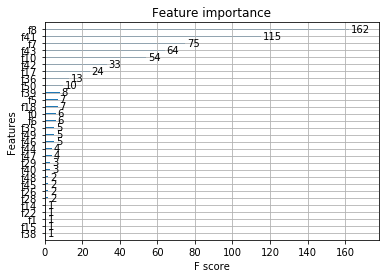
\includegraphics[scale=0.5]{comparison_between_features.png}
	\caption{Comparison of importance between our initial set of features}
\end{figure}

In these partial models, the following features typically show higher importance over the others from selected index: \textit{Average sales customer number Ratio, Day of week, Number of Customers, School Holiday, Month In Promotion, promotion Interval, Average Sales, competition Day Count, Variance SC Ratio, promotion Day Count, Sales Variance.}\\
\\
We wrote two helper functions to get the important features using self-defined importance score threshold. However, after adjusting the threshold and parameter tuning, we find that the partial model does not show significant improvement, meaning the existing full features already works quite well. 

\begin{center}
 \begin{tabular}{||c c c c c c c||} 
 \hline
 Model Name & 1st CV & 2nd CV & 3rd CV & 4th CV & 5th CV & Average CV Error \\ [0.5ex] 
 \hline\hline
 Partial Full Model & 0.109 & 0.174 & 0.094 & 0.092 & 0.068 & 0.107 \\ 
 \hline
 Partial Logged Model & 0.123 & 0.153 & 0.078 & 0.078 & 0.078 & 0.102 \\ 
 \hline
 Partial Ratio Model & 0.074 & 0.070 & 0.075 & 0.092 & 0.062 & 0.075 \\ [1ex] 
 \hline
\end{tabular}
\end{center}

\subsection{Ensemble regression method}

Since xgboost model may have its own assumptions and biases, we experimented other SKLearn’s models. Using the same set of full features on normal, log and ratio data, those models below works relatively well even though no single model can beat XGB’s Ratio model with error of 0.075.\\
\\
As there are intrinsic assumptions behind each model, and some of these assumption can slightly affect the prediction, we have shortlisted the following models’ predictions as they generally have lower cross validation error (smaller than 0.12 as our threshold) and they are consistent in sample predictions: \\

\textit{XGBRatioModel, XGBPartialRatioModel, XGBLoggedModel, XGBPartialModel, XGBPartialLoggedModel, adaBoostRatioModel, BaggingFullModel, BaggingLoggedModel, BaggingRatioModel, ExtraTreeRatioModel, GradientBoostingLoggedModel, GradientBoostingRatioModel, RandomForestFullModel, RandomForestLoggedModel, RandomForestRatioModel}\\

Averaging arithmetically all of the above model’s prediction, we get our final prediction. According to our cross validation, we are confident that the out of sample error will be contained within 0.10.


\begin{center}
 \begin{tabular}{||c c c c c c c||} 
 \hline
 Model Name & 1st CV & 2nd CV & 3rd CV & 4th CV & 5th CV & Average CV Error \\ [0.5ex] 
 \hline\hline
 AdaBoost Full Model & 0.212 & 0.453 & 0.295 & 0.291 & 0.262 & 0.302 \\ 
 \hline
 AdaBoost Logged Model & 0.165 & 0.350 & 0.190 & 0.205 & 0.173 & 0.217 \\ 
 \hline
 AdaBoost Ratio Model & 0.086 & 0.083 & 0.095 & 0.119 & 0.090 & 0.095 \\ 
 \hline
  Bagging Full Model & 0.096 & 0.161 & 0.090 & 0.097 & 0.066 & 0.102 \\ 
 \hline
  Bagging Logged Model & 0.096 & 0.172 & 0.082 & 0.093 & 0.066 & 0.102 \\ 
 \hline
  Bagging Ratio Model & 0.074 & 0.084 & 0.087 & 0.086 & 0.061 & 0.078 \\ 
 \hline
  Extra Tree Full Model & 0.135 & 0.207 & 0.130 & 0.103 & 0.071 & 0.129 \\ 
 \hline
  Extra Tree Logged Model & 0.123 & 0.202 & 0.129 & 0.098 & 0.070 & 0.125 \\ 
 \hline
  Extra Tree Ratio Model & 0.077 & 0.090 & 0.091 & 0.088 & 0.072 & 0.084 \\ 
 \hline
   Gradient Boosting Full Model & 0.120 & 0.174 & 0.122 & 0.126 & 0.081 & 0.125 \\ 
 \hline
   Gradient Boosting Logged Model & 0.011 & 0.151 & 0.103 & 0.105 & 0.070 & 0.108 \\ 
 \hline
   Gradient Boosting Ratio Model & 0.073 & 0.073 & 0.083 & 0.097 & 0.061 & 0.077 \\ 
 \hline
   Random Forest Full Model & 0.098 & 0.161 & 0.085 & 0.096 & 0.065 & 0.101 \\ 
 \hline
   Random Forest Logged Model & 0.095 & 0.173 & 0.080 & 0.092 & 0.065 & 0.101 \\ 
 \hline
   Random Forest Ratio Model & 0.074 & 0.083 & 0.087 & 0.086 & 0.060 & 0.078 \\ [1ex] 
 \hline
\end{tabular}
\end{center}

\section{Conclusion and future work}

In conclusion, using $sales/customer$ ratio as the new label significantly improves our prediction in all models. However, due to the small dataset that we have, our model could not predict special conditions that happen outside our sample, such as the effect of renovating the store. Our attempt in selecting features did not show significant improvement. However, it is possible that if we examine more combination of the features, we might be able to find a smaller set of features that is sufficient to capture the trend.

\newpage

\section{Statement of team's work}

We $<A0148008J, A0141132B>$, as a team, certify that we have followed the CS3244 Machine Learning class guidelines for homework assignments.  In particular, we expressly vow that we have followed the Facebook rule in discussing with others in doing the assignment and did not take notes (digital or printed) from the discussions.  


\section{References}
\url{https://stackoverflow.com/questions/34178287/difference-between-objective-and-feval-in-xgboost}\\
\url{https://github.com/dmlc/xgboost/blob/master/demo/guide-python/custom_objective.py}\\
\url{http://blog.kaggle.com/2017/05/19/march-machine-learning-mania-1st-place-winners-interview-andrew-landgraf}\\


\end{document}